\section*{Question 3}
The process
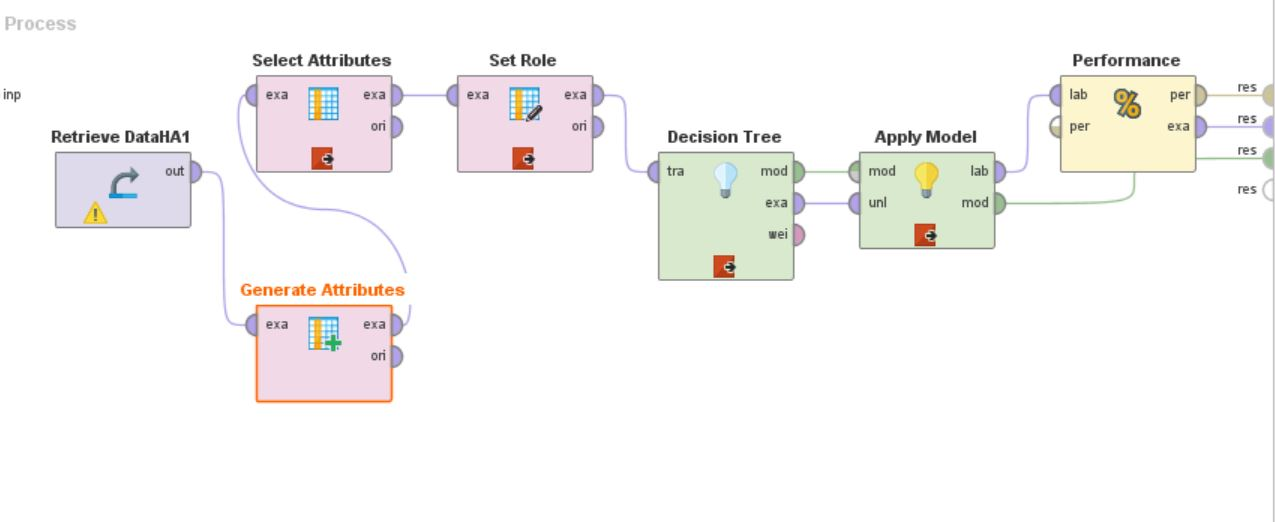
\includegraphics[width=0.8\textwidth]{Question3Process.jpg}

first changes the numerical attribute TotalActivites to a nominal one by
\textbf{Generate Attributes} and \textbf{Select Attributes}. The generating
consideres the old TotalActivites and contains the rule that all data, where
TotalActivites is lower or the same as 40 it should be assigned to ``Low''
otherwise ``High''. The \textbf{Set Role} gives the new attribute as label, so
RapidMiner knows what should have be the outcome of the Decision Tree.
\textbf{Decision Tree} generates the decision Tree. Then \textbf{Apply Model}
for \textbf{Performance} checking. The output is then the model and the
performance of the model on the data.

The found decision tree is 

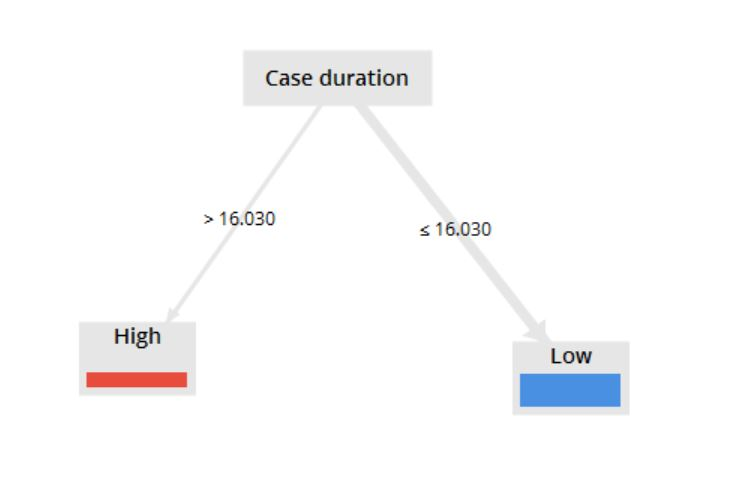
\includegraphics[width=0.8\textwidth]{Question3Deci.jpg}

If you check the Confusionmatrix

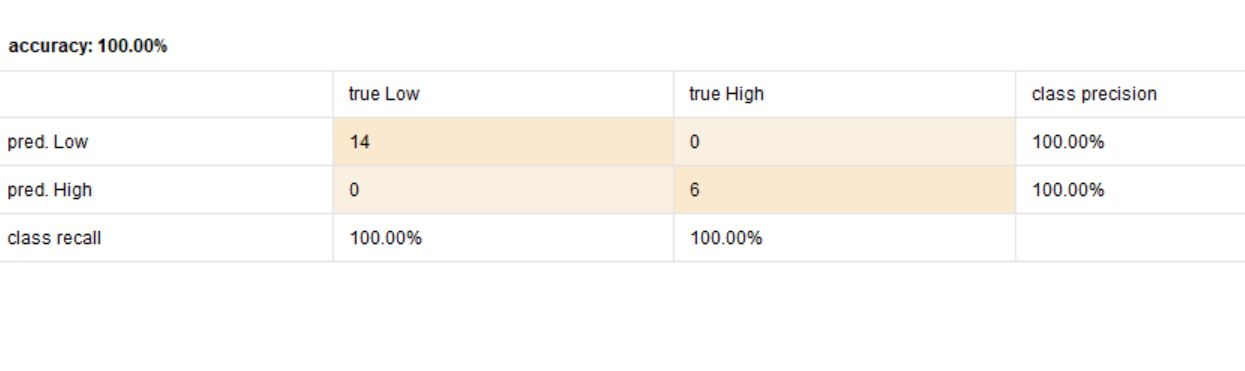
\includegraphics[width=0.8\textwidth]{Question3Confusion.jpg}

you see, that this decision tree classifys the data perfectly. So you can
predict by just knowing the case duration the total activities. If the case
duration is higher, than also the total activities are high. This seems to be
logical, if you have to do a lot this takes most of the times longer and
otherwise around, if you do not need long you mostly did not do a lot of
different things in the time.